\documentclass[conference]{IEEEtran}
\IEEEoverridecommandlockouts
% The preceding line is only needed to identify funding in the first footnote. If that is unneeded, please comment it out.
\usepackage{cite}
\usepackage{amsmath,amssymb,amsfonts}
\usepackage{algorithmic}
\usepackage{graphicx}
\usepackage{textcomp}
\usepackage{hyperref}
\usepackage{xcolor}
\def\BibTeX{{\rm B\kern-.05em{\sc i\kern-.025em b}\kern-.08em
    T\kern-.1667em\lower.7ex\hbox{E}\kern-.125emX}}
\begin{document}

\title{The Observatory}

\author{\IEEEauthorblockN{1\textsuperscript{st} Fabio Plunser}
    \and
    \IEEEauthorblockN{2\textsuperscript{nd} Dominik Barbist}
    \and
    \IEEEauthorblockN{3\textsuperscript{rd} Florian Gruber}
}

\maketitle

\section{Introduction}
For this project, we need to implement a system that can detect unknown faces in a given environment (IoT device/cameras).
For that, it will use a camera to collect images, process them on the edge device, and send the processed images to the cloud.
In the cloud, we will use Amazon Rekognition to analyze the faces and compare them with a database (S3) of known faces.
If an unknown face is detected, we will send a signal to the edge device to trigger an alarm for the responding IoT device.
A high level of parallelism is needed to process the images sent from at least 5 video sources.
\\
\textbf{Main Steps:}
\begin{itemize}
    \item \textbf{Data Collection:} We need to collect images from the sensors and send them over the edge device to the cloud.
    \item \textbf{Data Processing:} We need to do preprocessing on the images to extract the relevant information (faces) on the edge device.
    \item \textbf{Data Storage:} We need to store the processed images in the cloud (S3).
    \item \textbf{Data Analysis:} We need to analyze the faces in the cloud and cross-reference them with faces in the database.
    \item \textbf{Signal Processing:} We need to send a signal to the edge device to notify the IoT device about an unknown face and subsequently trigger an alarm.
    \item \textbf{User Interface:} We need to provide a user interface for the user to view the unknown faces (maybe) and disarm the alarm.
\end{itemize}

\section{System architecture}
\begin{itemize}
    \item \textbf{Data Collection:} The main data collection will be consisting of video sequences from 6 different cameras provided by the WiseNet dataset.
          For the emulation of the cameras, we will use a nginx server running in a docker container. This setup will
          enable us to also use a real camera feed from a rtmp stream, which will give a more realistic setup.
    \item \textbf{Data Processing:} For the data preprocessing, we will use OpenCV, and for the face recognition, we will use YOLO(not sure about the exact version).
    \item \textbf{Data Storage:} We will use AWS S3 to store the processed images.To save bandwidth, we will only store(required for Amazon Rekognition) the processed images (faces)
          and not the raw images. To keep track of the processed images, we will use a database to link an IoT device with their processed images.
    \item \textbf{Data Analysis:} After the images are stored in S3, the edge device will send a signal to a Lambda function which will trigger the face recognition
          process in Amazon Rekognition.
    \item \textbf{Signal Processing:} If an unknown face is detected, the Lambda function will send a signal to the edge device to trigger an alarm for a given IoT device.
    \item \textbf{User Interface:} We will use a simple web interface to display the unknown faces(maybe) and disarm the alarm.
\end{itemize}
% Describe your system in detail, including a figure for your architectural diagram (IoT, Edge, Cloud layers, components developed and services used).

\begin{figure}[h!]
    \centering
    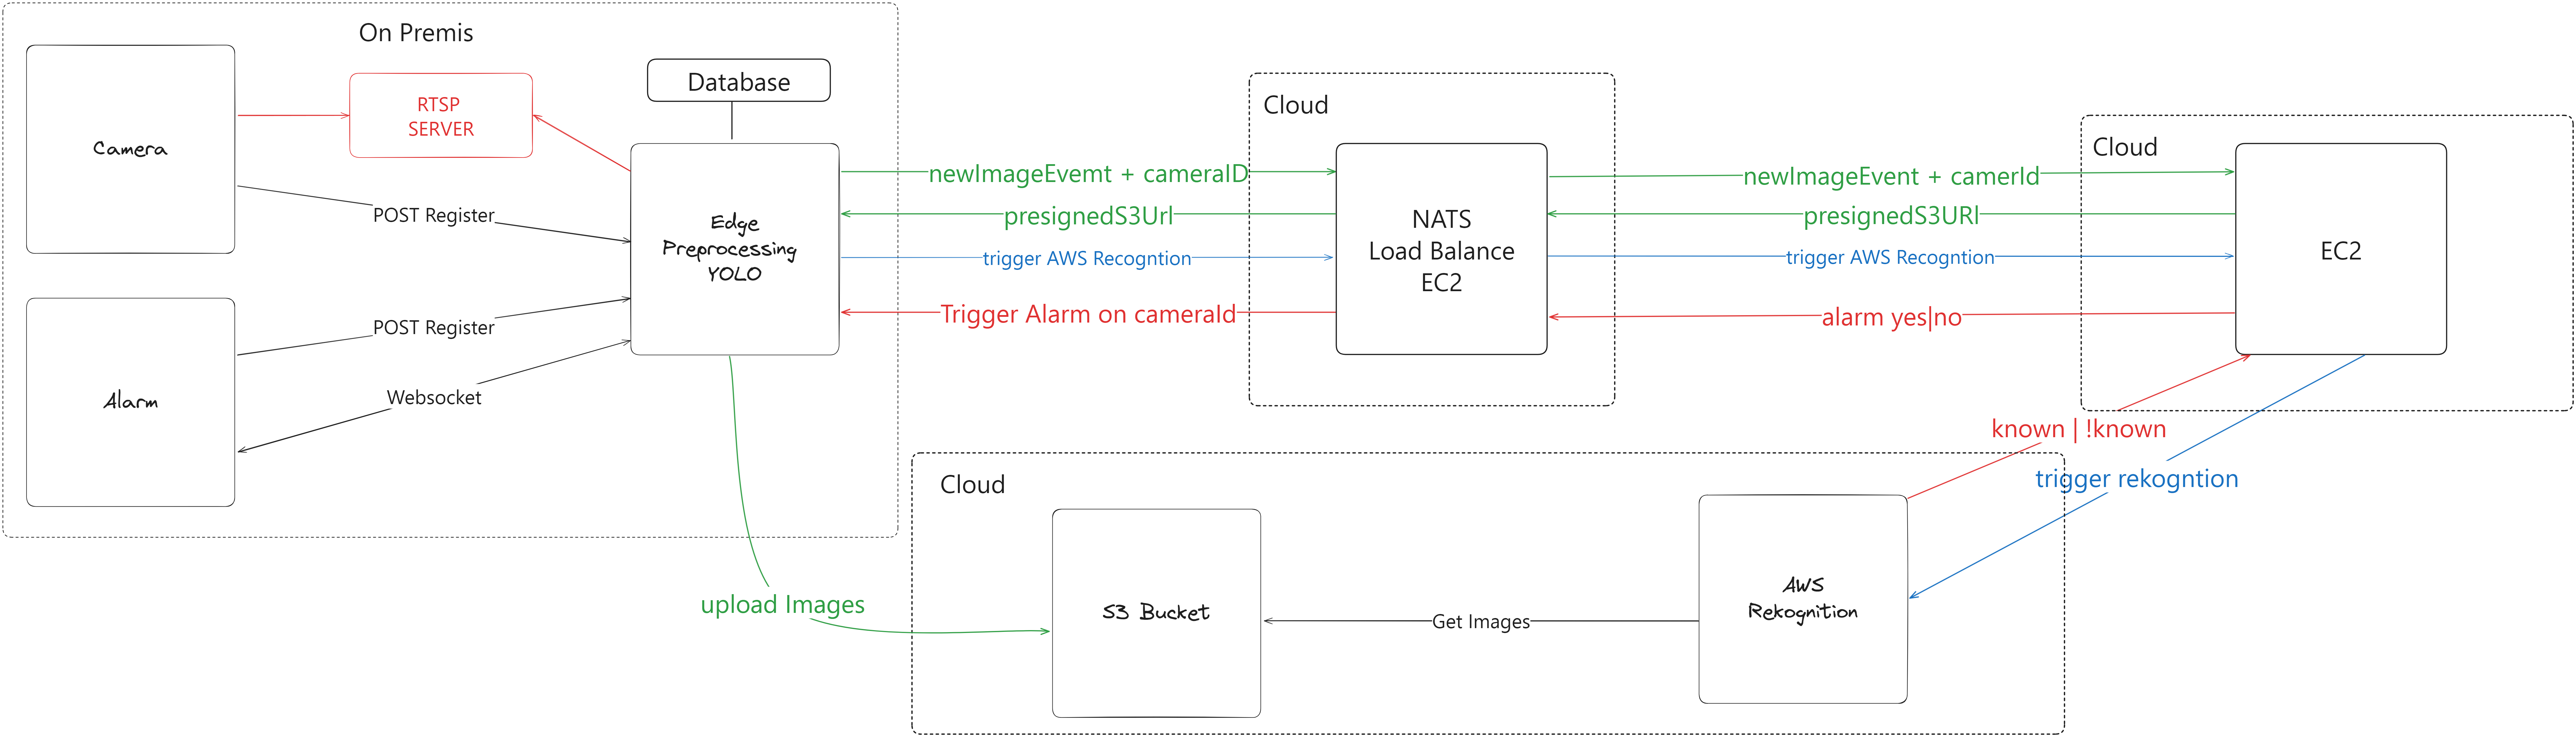
\includegraphics[width=1\linewidth]{images/architecturev2.excalidraw.png}
    \caption{Prototype of the system architecture.}
    \label{fig:enter-label}
\end{figure}


\section{Implementation details}
\subsection{Data Collection}
\begin{itemize}
    \item \textbf{Nginx-RTMP:} For the data transfer from the iot devices to the edge device we use a nginx server running in a docker container on aws ecs.
          The docker image "tiangolo/nginx-rtmp" is used for this purpose. In addition to the image, we also use the "nginx.conf" file to configure the server.
          The docker image can ether be run locally or on a aws ecs instance(See readme file in the iot folder for the exact setup).
    \item \textbf{WiseNet:} The dataset consists of 6 different camera feeds. We will use the iot.py script to send the 6 different camera feeds over the nginx server to the edge device.
          Each of the cameras have 11 different video sequences(except of one), after all the video sequences are played, the cameras will start again from the beginning.
          The data set itself will not be provided in the report materials, but can be found in the WiseNet dataset.
    \item \textbf{Camera:} In addition to the WiseNet dataset, we can also use a real camera feed from a rtmp stream. At the moment the each simulated camera has an hardcoded rtmp stream, in later
          stages of the project we will add a way for the cameras to register themselves to the onPremise server and get a rtmp stream assigned.
    \item \textbf{Edge:} The Edge device will receive the video feeds from the cameras and process them. The edge device will be a simple python script that will receive the video feeds from the cameras
          and process them. The processed images will be sent to the cloud for further processing.
\end{itemize}
\subsection{Data Processing}
\begin{itemize}
    \item \textbf{OpenCV:} Receiving and processing multiple camera feeds in real-time requires a substantial amount of computational power.
          So we decided to use a Load Balancer to distribute the load to multiple edge devices.
          Each of the edge devices will compare the previous frame with the current frame to detect if soothing has changed in the frame.
          Only if something has changed in the frame, the frame will be further processed to detect faces.
    \item \textbf{YOLO:} For the face detection we will use YOLO(not sure about the exact version). YOLO is a real-time object detection system that can detect objects in images and videos.
          We will use YOLO to detect faces in the images and send the processed images to the cloud. It is running on the on premise edge server which gets the video feeds to only
          send images to cloud if a face is detected. 
          The YOLO version we will use is version 11. This version contains 5 different models, with different sizes and speeds. The models are n, s, m, l, and x. 
          The model n is the smallest and fastest model, but also the least accurate. The model x is the largest and slowest model, but also the most accurate.
          See Section~\ref{sec:evaluation} for more details on the performance of the different models.
\end{itemize}
\subsection{Data Storage}
\begin{itemize}
    \item \textbf{AWS S3:} ...
    \item \textbf{Database:} ...
\end{itemize}
\subsection{Data Analysis}
\begin{itemize}
    \item \textbf{Amazon Rekognition:} ...
\end{itemize}
\subsection{Signal Processing}
\begin{itemize}
    \item \textbf{Lambda Function:} ...
    \item \textbf{NATS:} For the communication between on premise edges and the cloud we will be using NATS. NATS is a simple, secure and high performance open source messaging system for cloud native applications, IoT messaging, and microservices architectures.
          The on premise edge device will send a signal to the cloud to get a presigned URL for Wasabi. The presigned URL will be used to upload the processed images to the cloud.
          After the upload is finished the on premise server will send a nats message to the cloud which will trigger either a lambda function or ec2 instance to do the face recognition process. 
          The process is finished and the same lambda function or ec2 instance will send a nats message back to the on premise server to trigger the alarm.
\end{itemize}
\subsection{User Interface}
\begin{itemize}
    \item \textbf{Web Interface:} ...
    \item \textbf{Disarm Alarm:} ...
\end{itemize}

\section{Evaluation}
\label{sec:evaluation}
% Evaluation of the response time and scalability (number of devices and traffic) to prove the correctness of your implementation. 
% The more detailed the better. 

\end{document}
